\documentclass{article}
\usepackage{amsmath}
\usepackage{graphicx}

\title{Domino and Tromino Tiling}
\author{}
\date{}

\begin{document}

\maketitle

\section*{Problem Description}

You have two types of tiles: a $2 \times 1$ domino shape and a tromino shape. You may rotate these shapes.

\begin{center}
    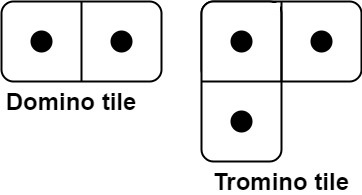
\includegraphics[width=0.4\textwidth]{lc-domino.jpg}
\end{center}

Given an integer $n$, return \emph{the number of ways to tile a $2 \times n$ board}. Since the answer may be very large, return it modulo $10^9 + 7$.

\section*{Constraints}

\[
1 \leq n \leq 1000
\]

\end{document}
